\documentclass[tikz,border=2pt]{standalone}
\usepackage{amsmath,amssymb}
\usepackage{tikz}
\usetikzlibrary{arrows.meta}

\begin{document}
% Y = g(X) = X^2 for X uniform on {-2,-1,0,1,2}: values that g sends to the same number pool
% their probabilities, so P(Y=1) = P(X=-1) + P(X=1) = 2/5.
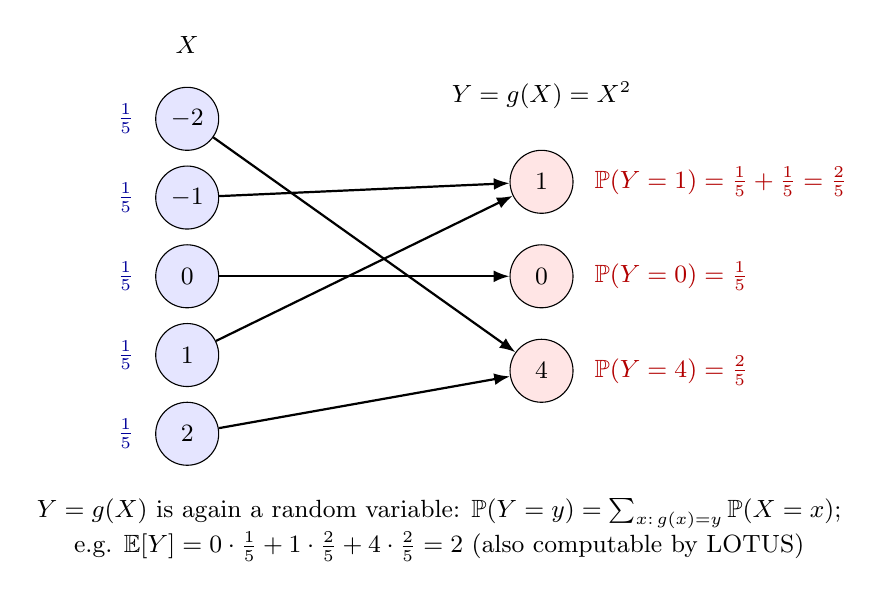
\begin{tikzpicture}[every node/.style={font=\small}, >={Latex[length=2mm]}]
	\foreach \y/\v in {4/-2, 3/-1, 2/0, 1/1, 0/2} {
		\node[draw, circle, fill=blue!10, minimum size=8mm] (x\y) at (0,\y*1.0) {$\v$};
		\node[anchor=east, font=\small, blue!60!black] at (-0.55,\y*1.0) {$\tfrac15$};
	}
	\node[draw, circle, fill=red!10, minimum size=8mm] (y0) at (4.5,2.0) {$0$};
	\node[draw, circle, fill=red!10, minimum size=8mm] (y1) at (4.5,3.2) {$1$};
	\node[draw, circle, fill=red!10, minimum size=8mm] (y4) at (4.5,0.8) {$4$};
	\draw[->, thick] (x2) -- (y0);
	\draw[->, thick] (x3) -- (y1);
	\draw[->, thick] (x1) -- (y1);
	\draw[->, thick] (x4) -- (y4);
	\draw[->, thick] (x0) -- (y4);
	\node[anchor=west, font=\small, red!70!black] at (5.05,2.0) {$\mathbb{P}(Y=0)=\tfrac15$};
	\node[anchor=west, font=\small, red!70!black] at (5.05,3.2) {$\mathbb{P}(Y=1)=\tfrac15+\tfrac15=\tfrac25$};
	\node[anchor=west, font=\small, red!70!black] at (5.05,0.8) {$\mathbb{P}(Y=4)=\tfrac25$};
	\node[anchor=south] at (0,4.7) {$X$};
	\node[anchor=south] at (4.5,4.0) {$Y=g(X)=X^2$};
	\node[anchor=north, align=center] at (3.2,-0.7) {$Y=g(X)$ is again a random variable: $\mathbb{P}(Y=y)=\sum_{x:\,g(x)=y}\mathbb{P}(X=x)$;\\ e.g. $\mathbb{E}[Y]=0\cdot\tfrac15+1\cdot\tfrac25+4\cdot\tfrac25=2$ (also computable by LOTUS)};
\end{tikzpicture}
\end{document}
